% $Date$
\documentclass[12pt,a4paper]{article}
\usepackage[polish]{babel}                      % Język polski
\usepackage[utf8]{inputenc}                     % Kodowanie dokumentu
\usepackage[T1]{fontenc}                        % Kodowanie fontów
%\usepackage{lmodern}
\usepackage{times}                              % Font wektorowy
\usepackage[cm]{fullpage}                       % Cała szerokość strony
\usepackage[pdftex,bookmarks,colorlinks]{hyperref} % Linki w dokumencie PDF
\usepackage{indentfirst}                        % Wcięcia akapitów
\usepackage{graphicx}                           % Grafika w png, jpeg, gif
%\pagestyle{headings}
%\graphicspath{{png}}                            % Szuka grafik w katalogu png
\frenchspacing                                  % Odstępy międzyzdaniowe

\title{ConvML 1.2}
\author{Marcin Kacprzak\\ marcin.kacprzak@entertech.com.pl\\
  \and Piotr Kulinowski\\ piotr.kulinowski@entertech.com.pl}
\date{\today}

\begin{document}

\maketitle

\begin{abstract}
  Ten dokument zawiera opis funkcji i składni języka ConvML.  ConvML jest językiem
  do zapisu strukturalnego modelu przenośnika taśmowego w formacie XML [XML10].

  Wersję PDF tego dokumentu można odnaleźć pod adresem
  \href{http://www.entertech.com.pl/convml/convml.pdf}{entertech.com.pl/convml/convml.pdf}.
\end{abstract}

\tableofcontents


\section{Wstęp}
Potrzeba opracowania modelu strukturalnego przenośnika taśmowego wynikła z
informatycznej konieczności wprowadzenia procedury zapisu pełnej informacji o
urządzeniu, która jednoznacznie i spójnie opisywałaby parametry
techniczno-ruchowe i konfigurację przenośnika taśmowego.  Ze względu na
uniwersalność zapisu i chęć popularyzacji modelu strukturalnego wprowadzono
anglojęzyczne nazewnictwo poszczególnych podzespołów.

Do opracowania systemu zapisu modelu strukturalnego przenośnika taśmowego
wykorzystano język XML Schema [XSD10], ułatwiający definiowanie struktury i
kolejności podzespołów przenośnika taśmowego (Tabela 4 1) oraz umożliwiający w
łatwy sposób jego adaptację na platformie informatycznej.  Istotną cechą modelu
strukturalnego jest praktycznie nieograniczona możliwość jego rozbudowy, bez
utraty przejrzystości struktury.  Każdy z elementów posiada grupę atrybutów
opisujących jego cechy, mogące być zarówno parametrami technicznymi jak i
ekonomicznymi.


\section{Konwencje}
Nazwa ConvML pochodzi od Conveyor Meta Language.  Typowy dokument ConvML ma
postać pliku tekstowego o rozszerzeniu xml lub convml.  Zalecane kodowanie to
UTF-8.

Dokument ConvML do zapisu informacji o strykturze przenośnika wykorzystuje
\emph{elementy}, a do zapisu właściwości używane są \emph{atrybuty} języka XML.
Elementy w języku ConvML mogą zawierać inne elementy oraz atrybuty, nie używa
się natomiast tekstu zawartego pomiędzy znacznikami do zapisu informacji o
przenośniku taśmowym.

Elementy języka ConvML należą do przestrzeni nazw:
http://www.entertech.com.pl/bcml.


\section{Struktura dokumentu}
Głównym elementem dokumentu jest ConvML.  Podelementy Meta oraz Types są
opcjonalne. Element BeltConveyor musi wystąpić co najmniej raz aby dokument był
poprawny.  Przykładowa instancja dokumentu może mieć następującą postać:

\begin{verbatim}
<?xml version="1.0" encoding="utf-8"?>
<ConvML version="1.2">
  <Meta />
  <Types />
  <BeltConveyor />
</ConvML>
\end{verbatim}  


\subsection{Element główny <ConvML>}

\begin{figure}[h]
  \centering
  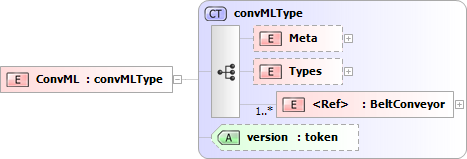
\includegraphics[width=0.6\textwidth]{png/convml_xsd2}
  \caption{Definicja elementu ConvML}
  \label{fig:convml-xsd}
\end{figure}

\paragraph{Definicje atrybutów:}
\begin{description}
\item[version] Zastosowana w dokumencie wersja języka ConvML.
\end{description}


\subsection{Przenośnik taśmowy <BeltConveyor>}
Górnicze przenośniki taśmowe definiuje się jako urządzenia służące do ciągłego
transportu na taśmie materiałów sypkich, pozyskiwanych podczas procesów
związanych z prowadzeniem robót górniczych [Kulinowski2011].  Do zespołów
głównych przenośnika taśmowego należą: stacja czołowa, stacja zwrotna, stacja
napinania taśmy, taśma, trasa, zestawy krążnikowe i krążniki [Antoniak2005].

\begin{figure}
  \centering
  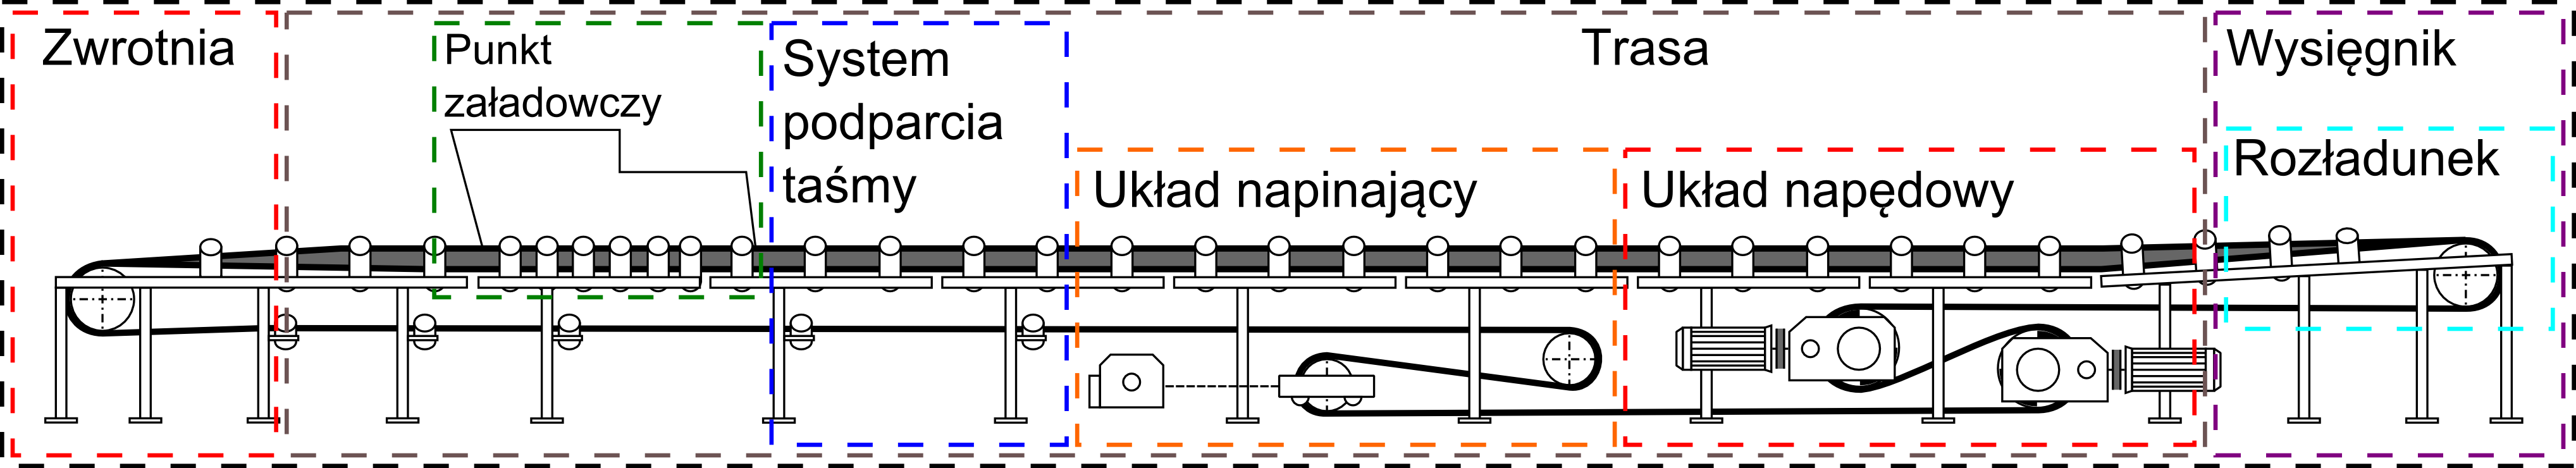
\includegraphics[width=\textwidth]{png/belt_conveyor_drw}
  \caption{Podstawowe podzespoły przenośnika taśmowego}
  \label{fig:przenosnik}
\end{figure}

W języku ConvML podstawowy podział przenośnika taśmowego wygląda następująco:

\begin{itemize}
\item Belt -- taśma,
\item Tail -- stacja zwrotna,
\item Route -- trasa,
\item Head -- stacja czołowa.
\end{itemize}

Pozostałe zespoły główne przenośnika taśmowego znajdują się głębiej w strukturze
opisywanej przez język ConvML.  System podparcia taśmy należy do elementów
składowych trasy.  Układy napędowy i napinający są powiązane z bębnami, które
mogą występować jako elementy składowe stacji zwrotnej, stacji czołowej lub
trasy.

\begin{figure}[h]
  \centering
  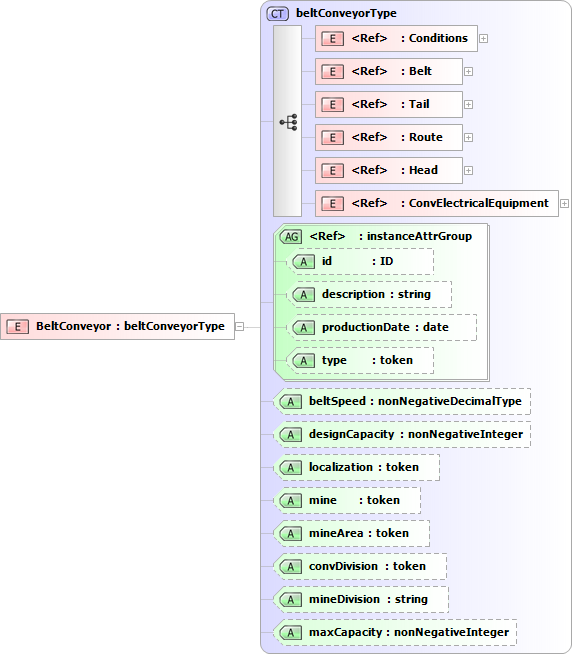
\includegraphics[width=0.6\textwidth]{png/belt_conveyor_xsd2}
  \caption{Definicja elementu BeltConveyor}
  \label{fig:belt-conveyor-xsd}
\end{figure}

\paragraph{Definicje atrybutów:}
\begin{description}
\item[beltSpeed] Prędkość taśmy przenośnika - v [m/s].
\item[designCapacity] Wydajność nominalna przenośnika - Q [t/h].
\item[localization] Wyrobisko.
\item[mine] Kopalnia.
\item[mineArea] Rejon.
\item[convDivision] Oddział taśmowy.
\item[mineDivision] Obsługiwane oddziały wydobywcze.
\item[maxCapacity] Wydajność maksymalna.
\end{description}

\subsection{Warunki pracy <Conditions>}
Element Conditions grupuje atrybuty związane z warunkami pracy przenośnika
taśmowego.

\begin{figure}[h]
  \centering
  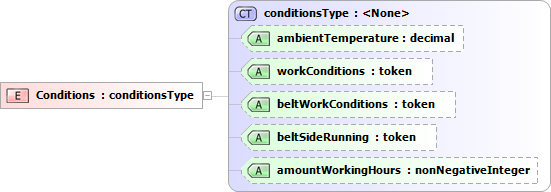
\includegraphics[width=0.6\textwidth]{png/conditions_xsd2}
  \caption{Definicja elementu Conditions}
  \label{fig:conditions-xsd}
\end{figure}

\paragraph{Definicje atrybutów:}
\begin{description}
\item[ambientTemperature] Temperatura otoczenia przenośnika - T [$^\circ$C].
\item[workConditions] Warunki pracy przenośnika: 1 - bardzo dobre, 2 - dobre,
  3 - przeciętne, 4 - ciężkie.
\item[beltWorkConditions] Warunki eksploatacji taśmy: 1 - bardzo dobre,
  2 - dobre, 3 - przeciętne, 4 - ciężkie.
\item[beltSideRunning] Zbieganie boczne taśmy: 1 - brak, 2 - małe, 3 - średnie,
  4 - duże.
\item[amountWorkingHours] Ilość godzin pracy przenośnika w ciągu roku [h].
\end{description}

\end{document}
